\begin{figure}[!htbp]
\centering
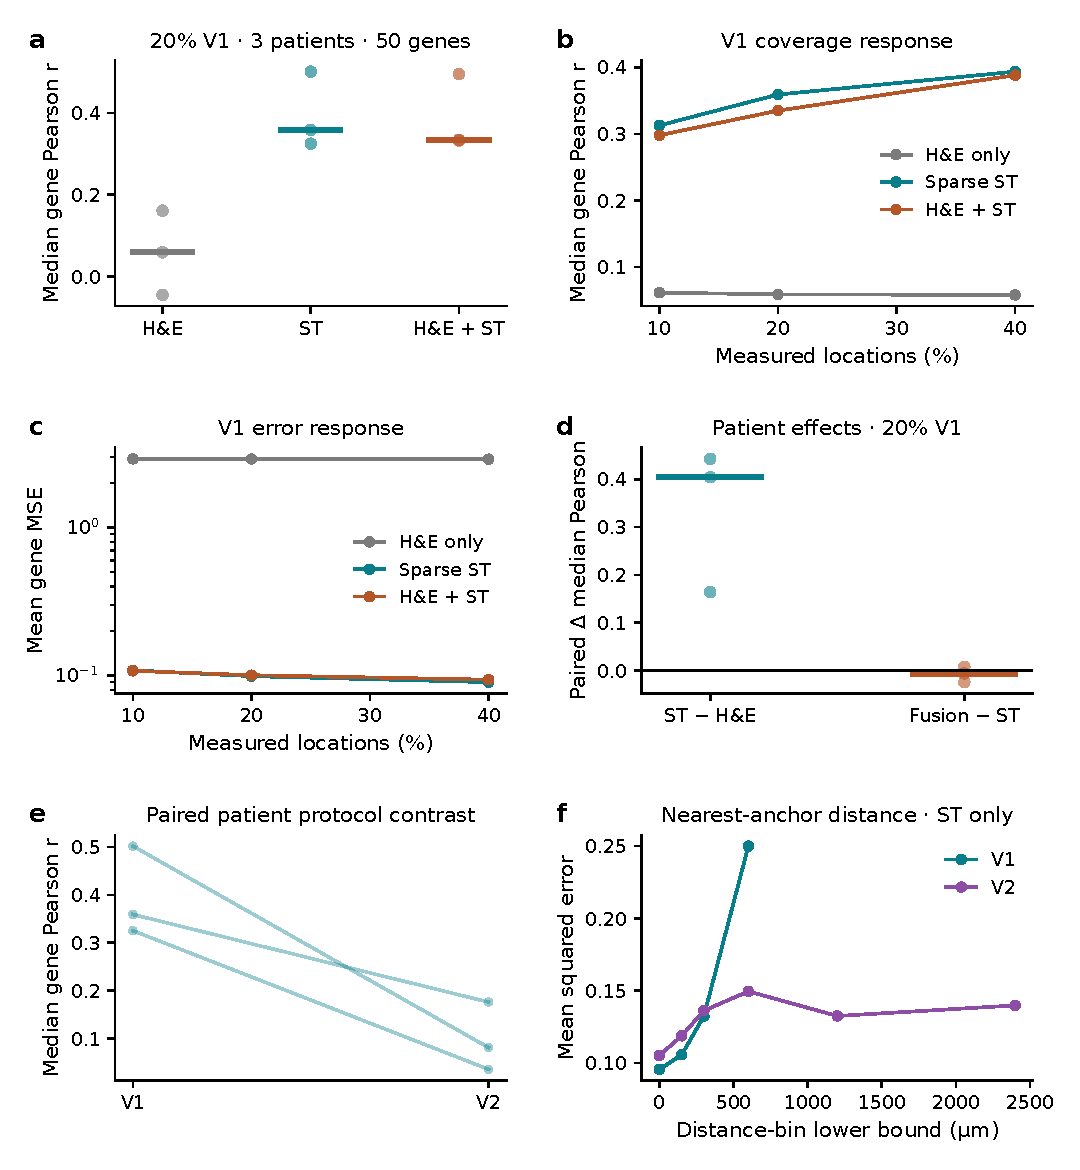
\includegraphics[width=\textwidth,height=0.70\textheight,keepaspectratio]{figures/Figure4.pdf}
\caption{\textbf{Fresh evaluation in three held-out Wu patients supports interpolation but not robust image fusion.} The frozen 50-gene panel was evaluated in patients 1160920F, CID4290 and CID44971, none of whom contributed to Wu calibration. \textbf{a,} Patient-level correlation summaries at 20\% distributed coverage. \textbf{b,c,} Median patient correlation and MSE across 10\%, 20\% and 40\% distributed coverage. \textbf{d,} Paired patient correlation effects for interpolation versus image-only prediction and fusion versus interpolation. \textbf{e,} Paired distributed (V1) and contiguous-region (V2) molecular correlations at 20\%. \textbf{f,} Distance-resolved molecular MSE at 20\%. Patient summaries average ten random mask seeds within geometry and then geometry means; cohort summaries are medians, not pooled spot estimates. Three fixed contiguous geometries are used for V2. Each patient is a biological replicate; seeds are not. V1 uses inverse-distance-squared interpolation and V2 uses a nearest-anchor mean, so panel e is a protocol contrast. The public image inputs contained only 15 or 25 native pixels per 112-\um{} patch, limiting conclusions about morphology. Error units are common development-standardized log1p counts.}
\label{fig:wu}
\end{figure}
